\documentclass{edpsci}
\usepackage{amsmath,amssymb,graphicx,booktabs,microtype}
\usepackage{etoolbox}
\usepackage[switch,mathlines]{lineno}
\usepackage[numbers,sort&compress]{natbib}
\usepackage{hyperref}
\usepackage{url}
\urlstyle{rm}
\graphicspath{{figures/}}
\hypersetup{colorlinks=true,citecolor=blue,urlcolor=blue,linkcolor=blue}
\journalname{Acta Acustica}
\renewcommand{\submittedto}{Template preview for}
\articletype{Research article -- preprint}
\hypersetup{pdftitle={Effects of arrival timing, source startup and room reflections on three-microphone sound localization},pdfauthor={Aneesh Arnav Chikkala},pdfsubject={Acta Acustica template preview; unreviewed preprint; not submitted}}
% Keep the supplied class intact; accommodate its header and one unaffiliated author.
\makeatletter
\patchcmd{\@maketitle}{\vbox to 22.7mm}{\vbox to 27mm}{}{\errmessage{EDP title-box patch failed}}
\patchcmd{\makeheadbox}{\vbox to0pt}{\vbox}{}{\errmessage{EDP article-band patch failed}}
\renewcommand{\institutename}{\par\begingroup\parindent=0pt\noindent\@institute\par\endgroup}
\makeatother
% The class uses \doi for article metadata; bibliography entries need a printed DOI.
\renewcommand{\doi}[1]{doi: \href{https://doi.org/#1}{\nolinkurl{#1}}}

\begin{document}
\title{Effects of arrival timing, source startup and room reflections on three-microphone sound localization}
\titlerunning{Arrival timing and source startup in sound localization}
\author{Aneesh Arnav Chikkala}
\authorrunning{Aneesh Arnav Chikkala}
\institute{No institutional affiliation}
\date{8 September 2026}
\abstract{Three-microphone sound localization estimates source direction from the small differences in arrival time between microphone signals. In a compact array, these differences are only a few microseconds, making the estimate sensitive to sampling, noise and reflected sound. Indoors, delayed reflections can produce stronger correlation peaks than the direct path. This limits small directional systems used in assistive hearing, mobile robots, voice control and acoustic monitoring. I examined arrival-time rounding, source startup and room reflections using GCC-PHAT simulations of an equilateral array with a 5~cm radius across three rectangular rooms. Root-mean-square error (RMSE) represents the typical angular miss, with lower values indicating better localization. At 10~dB SNR, rounding arrivals to the nearest sample increased direct-path RMSE from \(0.92^\circ\) to \(2.30^\circ\). In the most reflective test subset, starting the source and recording together produced a first-frame RMSE of \(4.16^\circ\), but allowing reflected sound to build before recording increased it to \(42.51^\circ\). Averaging 128 frames, or 5.46~seconds of audio, reduced error to \(0.84^\circ\) in the low-reverberation subset and \(10.16^\circ\) in the high-reverberation subset. These results show how unrealistic timing and startup assumptions can make a localization system appear more accurate than it would be during continuous indoor operation.}
\keywords{Sound localization, microphone arrays, GCC-PHAT, room simulation, arrival timing, source startup}
\maketitle
\raggedbottom
\linenumbers

\section{Introduction}
Sound localization becomes difficult when the microphone array is small because the useful time differences are also small. Noise and reflected sound can then hide or shift the direct-path delay. In this work, I use three microphones with generalized cross-correlation and phase transform (GCC-PHAT), treating the array geometry and the delay estimator as parts of the same system rather than independent design choices.

At 48~kHz, two consecutive samples are $20.83\,\mu$s apart. Sound travels about 7.15~mm in that time at 343~m/s, which is not negligible beside the 86.6~mm microphone spacing used here. Directly rounding every arrival to its nearest sample can therefore move the estimate by a meaningful fraction of the available inter-microphone delay.

Simulation makes it possible to separate delay rounding, source onset and reverberation, but only if the recording history is stated clearly. When analysis begins at the same instant as the source, the direct sound arrives before the reflected field has had time to develop. The first frame can then look far easier than the same scene under continuous operation.

Generalized cross-correlation is an established time-delay estimator \citep{knapp}, and GCC-PHAT has previously been applied to equilateral three-microphone arrays \citep{catur}. Fractional-delay filters provide a way of placing arrivals between samples \citep{laakso}, while the image-source method models reflections through mirrored sources \citep{allen}. I combine these established components to make a controlled comparison of arrival construction, source history and reflected propagation. I then test temporal averaging on a separate set of recordings instead of reusing the data from which its error model was estimated.

I checked the direct-path delays and room responses using independent numerical calculations, following the distinction between verifying an implementation and validating a physical system \citep{ernoult}. The analysis keeps the interactions between conditions and reports uncertainty for the fixed scenes used in the study. Its scope is deliberately narrow: one stationary synthetic source, three ideal matched microphones, three rectangular rooms and azimuth-only localization. Microphone calibration, hardware timing and accuracy in measured rooms require a separate experimental campaign.

\section{Simulation design and implementation}

\subsection{Microphone array and direction estimation}

The array places three microphones at the vertices of an equilateral triangle in the horizontal plane. Each microphone is 5 cm from the centre, giving an 8.66 cm spacing between microphones. I place the source 1.5 m from the centre at the same height. Figure~\ref{fig:geometry} shows this geometry and the matched comparisons used later in the study.

With azimuth measured counterclockwise from the positive $x$-axis, the microphone coordinates are
\begin{equation}
	\mathbf{m}_i
	=
	R[\cos\phi_i,\sin\phi_i]^T,
	\qquad
	\phi_i\in\{90^\circ,210^\circ,330^\circ\},
\end{equation}
where $R=0.05$ m. The speed of sound is fixed at $c=343$ m/s. For a source at $\mathbf{s}$, the direct-path arrival time at microphone $i$ is
\begin{equation}
	t_i=\frac{\lVert\mathbf{s}-\mathbf{m}_i\rVert}{c}.
\end{equation}
The time difference for pair $i,j$ is
\begin{equation}
	\tau_{ij}=t_i-t_j,\qquad i<j.
\end{equation}
The delay vector is ordered as
$\boldsymbol{\tau}=[\tau_{12},\tau_{13},\tau_{23}]^T$.
Although three pairs are available, their errors are correlated because the pairs share microphones.

Direction is estimated using a plane-wave model. For a unit vector $\mathbf{u}$ pointing toward the source,
\begin{equation}
	A\mathbf{u}=-c\boldsymbol{\tau},
\end{equation}
where each row of $A$ is $(\mathbf{m}_i-\mathbf{m}_j)^T$, ordered consistently with $\boldsymbol{\tau}$. The estimated delays give
\begin{equation}
	\widetilde{\mathbf{u}}
	=
	-cA^+\widehat{\boldsymbol{\tau}},
	\qquad
	\widehat{\theta}
	=
	\operatorname{atan2}
	(\widetilde{u}_y,\widetilde{u}_x),
	\label{eq:solve}
\end{equation}
where $A^+$ is the pseudoinverse. I use this equally weighted least-squares solution as a fixed estimator. It should not be read as a statistically optimal treatment of the pairwise errors, since the pairs share microphones and are therefore correlated. The vector itself is left unnormalised because only its angle is used.

The source is at a finite distance, so its wavefront is curved rather than planar. Even exact direct-path delays can therefore produce a non-zero angular error when passed through equation~\ref{eq:solve}. I quantify this model mismatch separately using analytical direct-path arrival times.

\begin{figure*}[t]
	\centering
	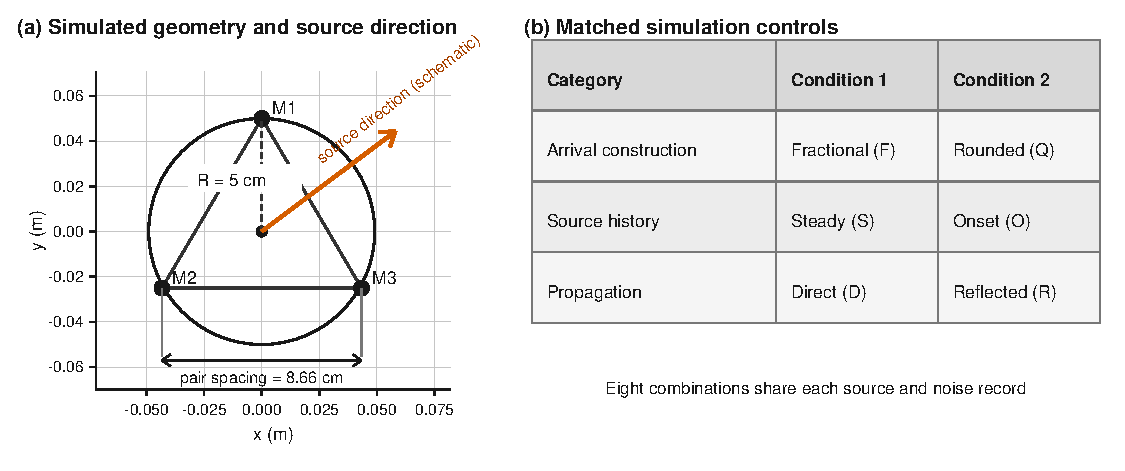
\includegraphics[width=\textwidth]{figures/fig1_geometry_controls.pdf}
	\caption{Microphone geometry and matched simulation controls. (a) Layout of the equilateral three-microphone array with circumradius $R=5$ cm and inter-microphone spacing of 8.66 cm. The microphone coordinates are drawn to scale; the arrow shows one tested source azimuth and is not drawn to the 1.5 m source distance. (b) The three matched binary controls form eight combinations. Within each scene and recording, every combination uses identical source and microphone-noise samples. ``Onset'' denotes one source startup at the beginning of the complete recording.}
	\label{fig:geometry}
\end{figure*}

\subsection{Room model and arrival timing}

I represent each room as a three-dimensional rectangular enclosure with specular reflections. The six walls use frequency-independent pressure-reflection coefficients. The model includes geometrical spreading but excludes diffraction, diffuse scattering, air attenuation and microphone directivity.

For room dimension $L_a$ and source coordinate $s_a$ along axis $a$, an image-source coordinate is
\begin{equation}
	s_a^{\mathrm{img}}
	=
	2n_aL_a+(1-2p_a)s_a,
\end{equation}
where $n_a\in[-K,K]$ and $p_a\in\{0,1\}$. The numbers of reflections at the low and high walls are $\lvert n_a-p_a\rvert$ and $\lvert n_a\rvert$, respectively. A path of length $r$ has an arrival time $r/c$ and pressure gain
\begin{equation}
	g(r)
	=
	\frac{1}{4\pi r}
	\prod_w\beta_w^{N_w},
\end{equation}
where $\beta_w$ is the pressure-reflection coefficient for wall $w$ and $N_w$ is the number of reflections from it. The final model uses $K=76$ and retains paths up to 1.2 s. I test convergence by repeating the room-response calculation with larger image extents and longer path limits.

For uniform walls, absorption is assigned using
\begin{equation}
	\alpha=\frac{0.161V}{S T_{\mathrm{nom}}},
	\qquad
	\beta=\sqrt{1-\alpha},
\end{equation}
where $V$ is room volume, $S$ is surface area and $T_{\mathrm{nom}}$ is the nominal reverberation setting. I measure the resulting decay from the simulated response instead of assuming that it equals $T_{\mathrm{nom}}$ \citep{bellows}.

I compare two ways of constructing arrival times. The fractional implementation first deposits each path linearly on a grid 32 times finer than the acquisition grid, then converts the response to the acquisition rate using a normalised Kaiser-windowed sinc filter. The Kaiser shape parameter is 8.6 and the filter half-width is 32 acquisition samples. The rounded implementation instead places each path at
\begin{equation}
	n=\operatorname{round}(f_s r/c).
\end{equation}
Everything else, including path gains, the reflection set and later signal processing, remains unchanged. This isolates the effect of replacing fractional arrivals with nearest-sample rounding. A direct-only condition removes the reflections while keeping the same direct path and response length.

\subsection{Source signal and recording procedure}

The source is a Gaussian random sequence restricted to 300--3400 Hz with a Fourier-domain mask and normalised by its root mean square amplitude. I use a 48 kHz sampling rate. Each continuous recording begins with a 59,682-sample pre-analysis interval, long enough to cover the 57,634-sample room response and one additional frame for the acquisition filter to settle. In the steady condition, the source is active throughout this interval. In the onset condition, it is zero before analysis begins.

All three microphone signals pass through the same causal Butterworth bandpass filter from 300 to 3400 Hz. The SciPy prototype order is four, producing four second-order sections and a total bandpass order of eight. I generate independent Gaussian noise for each microphone and pass it through the same filter.

Noise is scaled relative to the filtered, steady-state, direct-only signal. Let $P_{\mathrm{dir}}$ denote the direct-signal power averaged over the microphones and analysed samples, and let $P_{\mathrm{noise}}$ denote the corresponding acquired noise power. The reported SNR is
\begin{equation}
	\mathrm{SNR}
	=
	10\log_{10}
	\left(
	\frac{P_{\mathrm{dir}}}{P_{\mathrm{noise}}}
	\right).
\end{equation}
I retain the same noise samples and scaling after adding reflections. The stated SNR is therefore referenced to the direct sound, not to the total reverberant signal.

To examine source history, I match steady and onset recordings sample for sample. The source remains active through the pre-analysis interval in the steady recording. For the onset recording, I set only the earlier source samples to zero and leave the analysed source samples and microphone noise unchanged. The comparison includes both room-response buildup and causal-filter startup, so I treat it as a comparison between recording conditions rather than a pure reverberation effect. Direct-only results show which differences remain when reflections are removed.

Each short recording contains 32 consecutive, non-overlapping frames of 2048 samples. One frame lasts 42.667 ms and the full recording lasts 1.365 s. For temporal averaging, I use separate continuous recordings of 128 frames, or 5.46 s. Their frame estimates are combined by the circular average in Section~\ref{sec:averaging}, avoiding a false discontinuity at the azimuth wraparound boundary. I also tested an exploratory condition that restarts the source and acquisition history before every frame. Since this repeatedly samples the startup transient rather than continuous operation, I report it separately.

\subsection{Delay estimation using GCC-PHAT}

GCC-PHAT estimates each pairwise delay from the peak of a phase-weighted cross-correlation. I remove the mean from each frame, apply a symmetric Hann window and calculate a 4096-point Fourier transform. For microphone spectra $X_i[k]$ and $X_j[k]$, the cross spectrum is
\begin{equation}
	G_{ij}[k]=X_i[k]X_j^*[k].
\end{equation}
A denominator floor is applied before PHAT normalization:
\begin{linenomath}
\begin{align}
	d_{ij}[k]
	&=
	\max\bigl(\lvert G_{ij}[k]\rvert,q_{ij}\bigr),\\
	q_{ij}
	&=
	10^{-3}\max_l\lvert G_{ij}[l]\rvert+10^{-12},\\
	W_{ij}[k]
	&=
	G_{ij}[k]/d_{ij}[k].
\end{align}
\end{linenomath}
The maximum in $q_{ij}$ is taken over all frequency bins. I set $W_{ij}$ to zero outside 300--3400 Hz. The floor prevents unstable PHAT weights where the cross-spectrum magnitude is close to zero.

I evaluate the inverse transform on a correlation grid eight times finer than the acquisition grid. This interpolates the discrete correlation function; it does not add information to the microphone signals. The peak search is restricted to
\begin{equation}
	\lvert\tau_{ij}\rvert
	\leq
	\frac{\lVert\mathbf{m}_i-\mathbf{m}_j\rVert}{c}.
\end{equation}
A quadratic fit through the peak and its two neighbouring samples gives the final sub-grid estimate. I limit this correction to one correlation-grid interval and clip it to the physical delay bound. The three pairwise estimates are then passed to equation~\ref{eq:solve}.

\subsection{Measuring the simulated room response}

I calculate room decay after passing the impulse responses through the same causal 300--3400 Hz acquisition filter. The squared responses are reverse-integrated using Schroeder's method \citep{schroeder}, after summing energy across the three microphones. A line fitted between $-5$ and $-25$ dB is extrapolated to 60 dB to obtain T20. This value describes the band-limited simulated response. I also retain early decay time, T30 and goodness of fit to check whether the truncated response supports the fitted range.

The direct-to-reverberant ratio is calculated from separately filtered direct and reflected responses:
\begin{equation}
	\mathrm{DRR}
	=
	10\log_{10}
	\left(
	\frac{E_{\mathrm{dir}}}{E_{\mathrm{refl}}}
	\right).
\end{equation}
Both component energies are summed over microphones and time. I retain the interference term because the energy of the combined direct and reflected response is
\begin{equation}
	\begin{aligned}
	E_{\mathrm{tot}} &= E_{\mathrm{dir}}+E_{\mathrm{refl}}\\
	&\quad+2\sum_{i=1}^{3}\sum_n
	h_{\mathrm{dir},i}[n]h_{\mathrm{refl},i}[n],
	\end{aligned}
\end{equation}
where $h_{\mathrm{dir},i}$ and $h_{\mathrm{refl},i}$ are the filtered direct and reflected responses at microphone $i$.
For every scene, I record the arrival times and gains of the direct path and six first-order reflections. These values provide a direct check on room construction and help explain differences between the nominal setting and measured decay.

\section{Quality control and evaluation}

\subsection{Independent numerical checks}

I first test the direction calculation without room reflections. The analytical sweep compares exact spherical arrivals with rounded arrivals over 720 source angles, array radii of 0.025, 0.05 and 0.10 m, source distances of 0.5, 1.5, 5 and 20 m, and sampling rates of 16, 48, 96 and 192 kHz. Together, these produce 34,560 geometry and sampling conditions. Separate tests check plane-wave recovery across all 720 angles and three radii. I also use an independent scalar implementation to solve the two-dimensional normal equations at six selected angles for each radius and source distance, giving 72 spherical-reference comparisons. All six channel permutations are checked for one geometry and source direction using both analytical arrivals and waveform estimates, with the cardinal directions included as additional controls. These checks are separate from the full rounding sweep.

A separate direct-path calculation compares continuous-time harmonic signals against a sampled fractional-delay filter. Within each filter-refinement comparison, the bandwidth and observation interval are identical. Across sampling rates, I keep frame duration close to 42.667 ms by using the nearest whole number of samples. This check separates errors introduced while constructing the signal from those introduced while converting delay estimates into an azimuth.

I check the room model using an independent image-source enumeration in which every path is evaluated from its exact frequency-domain phase. This reference does not reuse the main path generator or its interpolation filter. I compare path counts, spectra and estimated directions for rooms with both uniform and unequal wall coefficients. Image extent is increased until two successive calculations differ by less than $0.05^\circ$ in direction, 1\% in T20 and 0.1\% in the probe-spectrum comparison. I then increase response duration and interpolation resolution separately and together, checking that neither truncation nor interpolation determines the result.

The $0.05^\circ$ criterion is a numerical convergence target for interpreting effects of roughly $0.5^\circ$ or more; it is not an accuracy requirement for an acoustic device. GCC-PHAT selects a peak, so convergence of the room response alone cannot guarantee that every random signal realization selects the same one. I therefore use separate, reproducible random-number seeds for the pilot and main evaluations.

\subsection{Test conditions and matched comparisons}

The three rooms measure $6\times5\times3$ m, $5\times4\times2.8$ m and $8\times6\times3.2$ m. Within each room, I place the array centre at coordinate fractions $(0.5,0.5,0.5)$ and $(0.6,0.45,0.5)$. The nominal reverberation settings are 0.15, 0.30 and 0.60 s. I use 12 source directions,
\begin{equation}
	\begin{aligned}
		\theta_j &= 7.37^\circ+30^\circ j,\\
		j &= 0,\ldots,11.
	\end{aligned}
\end{equation}
The minimum distance between any source or microphone and a wall is 0.312 m.

The main evaluation covers all 216 combinations of room, array placement, nominal reverberation setting and source direction. I evaluate each scene at 0, 10 and 20 dB SNR using five independent 32-frame simulations. Table~\ref{tab:protocol} gives the resulting number of frame-level estimates. The condition allocation and analysis rules were fixed before I examined the held-out results.

\begin{table}[t]
	\caption{Evaluation counts. Each frame contains 2048 samples. Pilot, reference and sensitivity calculations are additional.}
	\label{tab:protocol}
	\centering
	\small
	\begin{tabular}{@{}lrr@{}}
		\toprule
		Study & Base scenes & Estimates\\
		\midrule
		Main room study & 216 & 103,680\\
		Seven additional variants & 72 & 80,640\\
		Long realizations & 72 & 92,160\\
		\midrule
		Total & & 276,480\\
		\bottomrule
	\end{tabular}
\end{table}

For matched comparisons, I use two subsets. The low-reverberation/centred subset combines the centred array with the nominal 0.15-s setting. The high-reverberation/offset subset combines the offset array with the nominal 0.60-s setting. Across three rooms and 12 source directions, these conditions give 72 base scenes. Absorption and placement both change between the subsets, meaning that their difference describes a combined acoustic condition rather than reverberation time alone.

At 10 dB SNR, all eight combinations of fractional or rounded arrivals, steady or onset history, and direct-only or reflected propagation share the same five source and noise realizations. I reuse the fractional/steady/reflected condition from the main evaluation only when every input is identical. For each scene, five additional 128-frame recordings estimate bias and temporal dependence, while five separate 128-frame recordings form the held-out temporal-averaging set. None of these long recordings are reused from the pilot study or 32-frame evaluation.

\subsection{Additional geometry and method checks}

I use a fixed subset containing source directions $7.37^\circ$, $97.37^\circ$, $187.37^\circ$ and $277.37^\circ$ in each of the six conditions formed by three rooms and the two matched acoustic subsets. These 24 scenes test a $17^\circ$ array rotation, an unequal triangular array, unequal wall absorption and a narrower 300--1700 Hz source band. For the unequal triangle, I scale the first microphone's relative $y$ coordinate by 0.65 and recenter the array. For unequal walls, the absorption multipliers $(0.5,1.5,1,1,1,1)$ are applied to the low and high walls along $x$, $y$ and $z$. They are normalised to preserve area-weighted mean absorption before the coefficients are clipped to $[0.0001,0.99]$.

The acquisition filter and direction estimator keep their 300--3400 Hz passband when the source band is narrowed. Each variation uses five new 32-frame realizations at 10 dB SNR. These variations do not share the base condition's random inputs, so I treat them as sensitivity checks rather than matched estimates of individual causal effects.

I include steered-response power with phase-transform weighting (SRP-PHAT) as a second localization method \citep{dibiase}. It uses the same signals, frame window, frequency band and PHAT normalisation as GCC-PHAT. For pair $i,j$ and candidate azimuth $\theta$, define
\begin{equation}
	C_{ij}(\theta)
	=
	\sum_{k\in\mathcal{B}} W_{ij}[k]
	\exp\!\left[
	\mathrm{i}2\pi f_k\tau_{ij}(\theta)
	\right].
\end{equation}
The SRP-PHAT objective is then
\begin{equation}
	P(\theta)
	=
	\sum_{i<j}\operatorname{Re}
	\bigl\{C_{ij}(\theta)\bigr\}.
\end{equation}
Here $\mathcal{B}$ contains the frequency bins from 300 to 3400 Hz and $\tau_{ij}(\theta)$ is the plane-wave delay predicted for pair $i,j$. I evaluate the objective on a $0.25^\circ$ azimuth grid, refine it quadratically around its maximum and check the result against a $0.05^\circ$ grid. This is a restricted comparison on the stated subset, not a general ranking of localization methods.

\subsection{Error measures and uncertainty}

For true azimuth $\theta$ and estimate $\widehat{\theta}$, angular error is defined as
\begin{equation}
	e=
	\operatorname{wrap}_{[-180^\circ,180^\circ)}
	\bigl(\widehat{\theta}-\theta\bigr).
	\label{eq:error}
\end{equation}
This wrapping prevents a small crossing of the angular boundary from being counted as a large error. I summarise performance using root mean square error,
\begin{equation}
	\mathrm{RMSE}
	=
	\sqrt{
		\frac{1}{N}
		\sum_{n=1}^{N}e_n^2
	},
\end{equation}
together with median absolute error, the 90th percentile of absolute error, circular bias and the proportion of estimates whose absolute error exceeds $5^\circ$. This threshold is descriptive; it is not a hearing or device-acceptance standard.

I estimate uncertainty with 2000 bootstrap draws \citep{efron}. Within a scene, complete simulated recordings are sampled with replacement and all frames from a selected recording remain together. Matched variants receive the same bootstrap selection. This keeps the pairing between conditions and avoids treating frames from one recording as independent experiments. The intervals describe variation from the simulated source and microphone noise in these fixed scenes. They do not cover all possible rooms, and five independent recordings per scene limit their precision.

Matched effects are calculated before aggregation. For loss function $L$, the paired effect for recording $r$ is
\begin{equation}
	\Delta_r=L_{r,A}-L_{r,B}.
\end{equation}
Here $L$ is signed angular error or squared angular error. Mean squared error is averaged before taking its square root to obtain RMSE. I report a difference between two RMSE values only as a difference in summary performance, not as an independent error component.

Interactions are calculated as differences between paired effects. Let Q and F denote rounded and fractional arrival construction, and let $h\in\{\mathrm{S},\mathrm{O}\}$ denote steady and onset history. For propagation condition $q\in\{\mathrm{R},\mathrm{D}\}$, denoting reflected and direct-only propagation, define the rounding effect at each history as
\begin{equation}
	\Delta_{\mathrm{Q},h}^{(q)}
	=
	L_{\mathrm{Q},h,q}-L_{\mathrm{F},h,q}.
\end{equation}
The reported rounding-by-reflection interaction averages the difference of differences equally over the two histories:
\begin{equation}
	\Delta_{\mathrm{int}}
	=
	\frac{1}{2}\sum_{h\in\{\mathrm{S},\mathrm{O}\}}
	\left(\Delta_{\mathrm{Q},h}^{(\mathrm{R})}
	-\Delta_{\mathrm{Q},h}^{(\mathrm{D})}\right).
\end{equation}
This quantity asks whether the effect of arrival-time rounding changes once reflections are present. The onset-by-reflection interaction is calculated in the same way, averaging equally over fractional and rounded arrival construction. I form every contrast within its recording before averaging over recordings and fixed scenes, while retaining the per-scene results beside the pooled summaries.

\subsection{Testing averaging on held-out realizations}
\label{sec:averaging}

I evaluate temporal averaging on the five held-out 128-frame recordings for each scene. The averaging lengths are
\begin{equation}
	N\in\{1,2,4,8,16,32,64,128\}.
\end{equation}
For each value of $N$, every held-out recording is divided into $128/N$ non-overlapping blocks of $N$ consecutive frames. Within a block, I combine the estimates using the circular mean
\begin{equation}
	\overline{\theta}_N
	=
	\arg\!\left(
	\sum_{n=1}^{N}
	\exp\!\left[\mathrm{i}\widehat{\theta}_n\right]
	\right).
\end{equation}
The circular mean avoids a discontinuity at the $-180^\circ/180^\circ$ boundary; angles are converted to radians before evaluating the exponential. Each low or high subset contains 36 scenes and five held-out recordings per scene, giving $180\times128/N$ block estimates. During bootstrapping, all blocks from one recording remain together. At $N=128$, each recording contributes one 5.461-s block.

Let $e_n$ be the wrapped frame error from equation~\ref{eq:error}. When these errors are sufficiently concentrated, circular averaging can be approximated by averaging the scalar errors. The prediction assumes an approximately stationary error process with persistent mean $b$ and covariance $\gamma_\ell$ between errors separated by $\ell$ frames, where $\gamma_0$ is the frame-error variance. The finite-lag covariance contribution is
\begin{equation}
	A_N
	=
	\sum_{\ell=1}^{N-1}(N-\ell)\gamma_\ell.
\end{equation}
Using this finite-lag covariance term, the variance and mean squared error are
\begin{equation}
	\begin{aligned}
		V_N
		&=
		\frac{\gamma_0}{N}
		+\frac{2A_N}{N^2},\\
		\operatorname{MSE}(\overline{e}_N)
		&\simeq b^2+V_N.
	\end{aligned}
	\label{eq:variance}
\end{equation}
$A_N$ collects covariance from the non-zero lags. The bias remains, while $V_N$ describes fluctuations that may decrease with averaging. A stationary source position by itself does not make the estimation errors stationary.

I estimate bias and covariance separately for each scene using its five 128-frame estimation recordings. Their pooled circular mean error provides the bias estimate and approximates the scalar mean when errors are concentrated. Each recording is centred before calculating its autocovariance. This removes differences between recording means, but it may also remove slowly changing error. The fitted covariance should therefore be read as a finite-record approximation, not an unbiased estimate of the full stationary covariance. Covariances above lag 32 are set to zero. For $1\leq\ell\leq32$, I apply a Bartlett taper,
\begin{equation}
	w_\ell=1-\frac{\ell}{33}
\end{equation}
to reduce sampling variation at longer lags. Centering, truncation and tapering can themselves bias the prediction. A comparison model assumes independent frames by setting all non-zero-lag covariances to zero. I set any negative fitted variance to zero before taking its square root, although this safeguard says nothing about the accuracy of the covariance estimate.

I interpret equation~\ref{eq:variance} only for estimation-set results with a circular resultant of at least 0.95 and an absolute circular mean error no greater than $15^\circ$. These criteria were fixed before examining the held-out recordings. They restrict where the small-error approximation is used but remove no scene from the empirical held-out results, nor do they rule out rare large errors.

\section{Results}

\subsection{Numerical verification and correction of the room model}

The plane-wave recovery differed from the analytical solution by at most $5.7\times10^{-14}$ degrees. The independent scalar solver differed from the main direction solver by no more than $7.3\times10^{-12}$ degrees, while the largest difference between the continuous-time waveform reference and the selected fractional-delay filter was $3.7\times10^{-5}$ degrees. Increasing the correlation-sampling factor from 8 to 64 changed the direct-path estimates by at most $0.000495^\circ$.

For one selected scene, the final independent room calculation evaluated about 5.22 million paths per microphone at 12 probe frequencies. Against this reference, the main room model gave a relative probe-spectrum difference of $1.13\times10^{-5}$ and an angular difference of $0.000807^\circ$. Earlier settings exposed two clear problems: insufficient image coverage moved one direction estimate by more than $100^\circ$, and a coarse fractional-delay grid failed the spectral criterion. Those failures determined the final numerical settings. The supplement and reproduction guide retain the checks, correction history and per-frame results.

A joint convergence check after the initial full run found another problem. When response duration and image extent were increased together, ten of 960 estimates changed by more than $0.05^\circ$, with a maximum change of $0.16551^\circ$. I retained the original 0.9-s/extent-48 run for audit but excluded it from the results. The corrected model uses a 1.2-s response, image extent 76 and propagation factor 32. Extending both limits again, to 1.5 s and extent 96, reduced the maximum change to $0.01273^\circ$. I then reran the study with the same condition allocation and analysis rules, but new source and noise identities. For this reason, the original and corrected campaigns are not treated as a recording-level matched comparison. Every result below comes from the corrected run.

\begin{table}[t]
	\caption{Final numerical checks. Values are the largest changes in estimated angle under each check. The independent reference covers one scene at 12 probe frequencies. Joint duration/extent refinement covers six scenes and 960 frames; each remaining refinement covers 24 scenes and 3840 frames. These changes are not localization errors relative to the source.}
	\label{tab:verification}
	\centering
	\small
	\begin{tabular}{@{}lr@{}}
		\toprule
		Check & Change ($^\circ$)\\
		\midrule
		Independent full room reference & 0.000807\\
		Longer response and larger image extent & 0.012726\\
		Propagation grid 32 to 64 & 0.006965\\
		Image extent 76 to 84 & 0.000000\\
		GCC factor 8 to 16 & 0.025930\\
		SRP angular grid refinement & 0.002310\\
		\bottomrule
	\end{tabular}
\end{table}

Table~\ref{tab:verification} and Figure~\ref{fig:numerics} collect the final checks. On the fixed 24-scene subset, doubling propagation resolution changed the estimates by at most $0.006965^\circ$, while increasing image extent produced no change. Increasing the GCC correlation-sampling factor changed the estimates by at most $0.02593^\circ$, and refining the SRP angular grid changed them by at most $0.002310^\circ$. Every checked change remained below the $0.05^\circ$ target. This establishes convergence for the tested cases, but it is not a worst-case bound over every possible input.

\begin{figure*}[t]
	\centering
	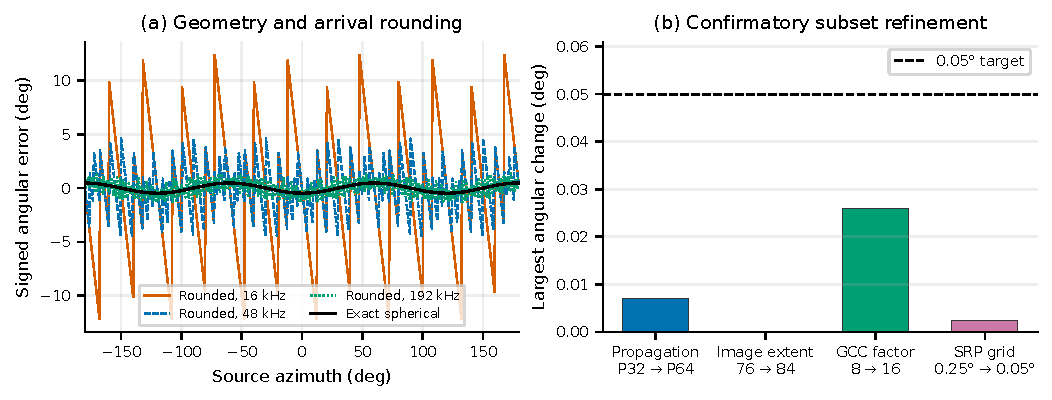
\includegraphics[width=\textwidth]{fig2_numerical_verification.pdf}
	\caption{Arrival-time rounding and numerical resolution. (a) Signed angular error relative to the true source azimuth for exact spherical arrivals and sample-rounded arrivals, with an array radius of 0.05 m and a source distance of 1.5 m. All curves use the same plane-wave direction solver and exclude waveform noise. The exact-spherical curve retains finite-distance curvature error; Figure~\ref{fig:precision}(a) isolates the additional rounding shift. (b) Largest angular changes under numerical refinement on the fixed 24-scene subset, using five recordings and 32 frames per scene. The dashed line marks the $0.05^\circ$ numerical target.}
	\label{fig:numerics}
\end{figure*}

For nominal settings of 0.15, 0.30 and 0.60 s, measured $T_{20}$ ranged from 0.083--0.110 s, 0.259--0.295 s and 0.586--0.683 s, respectively. The minimum fit $R^2$ was 0.928 in the lowest setting and 0.994 in the other two. Component direct-to-reverberant ratio (DRR) ranged from $-10.77$ to $+9.53$ dB. Since the nominal value specifies the absorption configuration rather than the measured decay, I report both quantities.

\subsection{Localization error across rooms}

At 10 dB SNR, RMSE increased from $1.620^\circ$ in the nominal-0.15-s setting to $11.954^\circ$ at 0.30 s and $37.233^\circ$ at 0.60 s. Their 95\% bootstrap intervals were $[1.599,1.641]^\circ$, $[11.168,12.771]^\circ$ and $[36.359,38.111]^\circ$. The proportion of estimates with more than $5^\circ$ absolute error also rose from 0.86\% to 27.38\% and 62.30\%.

At 20 dB SNR, the corresponding RMSE values were $1.362^\circ$, $11.796^\circ$ and $37.067^\circ$. Lower noise improved the least reflective condition, but it barely changed the larger errors in the other two. Figure~\ref{fig:core} shows the complete SNR range, including 0 dB, separately for each room.

Scene-level results reveal how much the pooled values hide. At 10 dB, RMSE ranged from $0.92^\circ$ to $3.16^\circ$ in the lowest setting, $2.08^\circ$ to $49.08^\circ$ in the middle setting and $6.56^\circ$ to $86.16^\circ$ in the highest setting. These ranges describe differences between the tested directions and array placements. They are not directly comparable to the bootstrap intervals around pooled RMSE, which measure resampling uncertainty within the fixed collection of scenes.

\begin{figure*}[t]
	\centering
	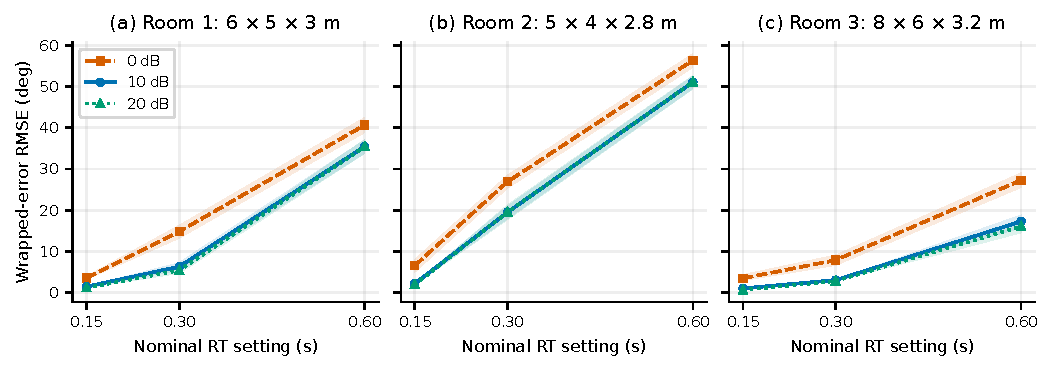
\includegraphics[width=\textwidth]{fig3_core_rooms.pdf}
	\caption{Main room results obtained with fractional arrivals and a source that was already running. Each point combines two array placements, 12 source directions and five 32-frame recordings. Shaded bands are 95\% record-bootstrap intervals for the fixed scenes. The horizontal axis shows the nominal setting used to select the wall absorption; $T_{20}$ was measured separately.}
	\label{fig:core}
\end{figure*}

\subsection{Effect of rounding arrival times}

Across the 72 matched scenes at 10 dB SNR, steady direct-path RMSE was $0.923^\circ$ $[0.912,0.934]^\circ$ with fractional arrivals and $2.300^\circ$ $[2.287,2.313]^\circ$ after rounding. The matched increase in mean squared error was $4.438\,\mathrm{deg}^2$ $[4.380,4.493]\,\mathrm{deg}^2$. The difference survives waveform construction, filtering and delay estimation; it is not limited to a calculation based on exact delays.

With reflections included, steady RMSE was $27.365^\circ$ for fractional arrivals and $28.112^\circ$ for rounded arrivals. The matched increase in mean squared error was $41.448\,\mathrm{deg}^2$ $[11.973,70.571]\,\mathrm{deg}^2$. The pooled increase is not uniform across scenes. Moving reflected paths between samples can change the selected cross-correlation peak, so the scene-level effect can vary in both magnitude and direction.

\subsection{Effect of source startup}

The strongest startup effect appears in the first analysed frame of the high-reverberation/offset subset. RMSE was $4.157^\circ$ when the source began immediately before acquisition and $42.508^\circ$ when it was already running. By the last frame of the 1.365-s recording, both matched conditions reached an RMSE of $41.526^\circ$. Earlier source history can no longer contribute at that point because the simulated response is finite. Figure~\ref{fig:paired} shows the two conditions converging as the reflected field develops.

Nothing in the algorithm changes between onset and steady conditions. The difference comes from the sound field presented to it. Restarting the source before every short observation repeatedly samples the brief period before reflections build up, which is not representative of continuous operation. The exploratory frame-reset check showed the same behaviour, but it used the pilot directions and is kept outside the main time trajectory.

Across all 72 scenes and 32 frames with fractional reflected signals, startup reduced mean squared error by $42.798\,\mathrm{deg}^2$, with a reduction interval of $[22.983,62.404]\,\mathrm{deg}^2$. Table~\ref{tab:effects} expresses the same result as the signed onset-minus-steady contrast, where a negative value means lower error at onset.

Using the complete factorial dataset, the onset-by-reflection interaction was $-49.046\,\mathrm{deg}^2$ $[-65.574,-32.891]\,\mathrm{deg}^2$ after averaging equally over fractional and rounded arrivals. The rounding-by-reflection interaction was $30.762\,\mathrm{deg}^2$ $[4.770,57.791]\,\mathrm{deg}^2$ after averaging equally over steady and onset histories. These non-zero interactions show that arrival construction, source history and reflected propagation do not behave as independent additive effects under the tested conditions.

\begin{table}[t]
	\caption{Matched changes in mean squared error ($\mathrm{deg}^2$) across 72 scenes at 10 dB. The rounding contrasts and the reflection contrast use steady recordings. The onset contrast uses fractional reflected signals and compares onset with steady operation over all 32 frames. Positive values indicate more error. Intervals resample complete recordings within each scene.}
	\label{tab:effects}
	\centering
	\small
	\begin{tabular}{@{}lrr@{}}
		\toprule
		Comparison & Change & 95\% interval\\
		\midrule
		Rounding, direct & 4.44 & [4.38, 4.49]\\
		Rounding, reflected & 41.45 & [11.97, 70.57]\\
		Onset, reflected & -42.80 & [-62.40, -22.98]\\
		Reflections, fractional & 747.97 & [699.52, 799.81]\\
		\bottomrule
	\end{tabular}
\end{table}

\begin{figure*}[t]
	\centering
	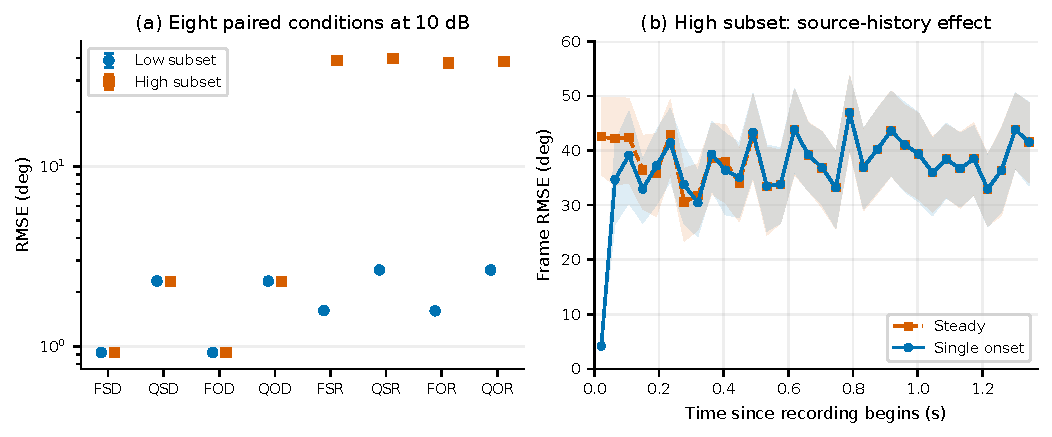
\includegraphics[width=\textwidth]{fig4_paired_attribution.pdf}
	\caption{Arrival construction and source startup at 10 dB. (a) All eight combinations. F and Q denote fractional and rounded arrivals, S and O denote steady and onset histories, and D and R denote direct and reflected propagation. The low and high subsets contain 36 scenes each and differ in both array placement and wall absorption. Error bars and shaded bands are 95\% intervals obtained by resampling complete recordings. (b) Matched fractional-arrival recordings with reflections in the high subset. In the steady condition, the source was already running when acquisition began. Markers indicate frame midpoints after the start of analysis.}
	\label{fig:paired}
\end{figure*}

\subsection{Improvement from temporal averaging}

Temporal averaging reduced block-level RMSE on the independent test recordings (Figure~\ref{fig:averaging}). In the low-reverberation/centred subset, it fell from $1.597^\circ$ $[1.584,1.610]^\circ$ for one frame to $0.835^\circ$ $[0.815,0.854]^\circ$ for 128 frames. In the high-reverberation/offset subset, it fell from $39.044^\circ$ $[38.439,39.607]^\circ$ to $10.158^\circ$ $[9.404,10.995]^\circ$. These results use the held-out averaging recordings and are not expected to match the frame-specific startup values. Even after 128 frames, 46.11\% of high-subset block estimates still exceeded $5^\circ$ absolute error.

Forty-nine of the 72 scenes met the estimation-set criteria for the small-error approximation. Their measured 128-frame test RMSE was $2.013^\circ$ $[1.932,2.090]^\circ$. The covariance-aware prediction was $2.075^\circ$, compared with $2.106^\circ$ under the independent-frame model. At shorter durations the agreement was weaker. The covariance model predicted $4.541^\circ$ against a measured $3.647^\circ$ for four frames, and $3.434^\circ$ against $2.844^\circ$ for eight, overpredicting by 24.5\% and 20.7\%. These comparisons remain descriptive because I did not calculate uncertainty intervals for the predictions. The small gap between the two 128-frame predictions is not enough to claim a practical advantage from covariance correction. Figure~\ref{fig:averaging} shows the complete duration-dependent result.

All 72 scenes remain in the empirical averaging curves. The restricted 49-scene analysis tests the approximation only where its estimation-set criteria were met and should not be read as complete test-set performance. Error after 5.46 s still varied between scenes and estimators. A finite observation cannot establish a universal or infinite-time reverberation limit.

\begin{figure*}[t]
	\centering
	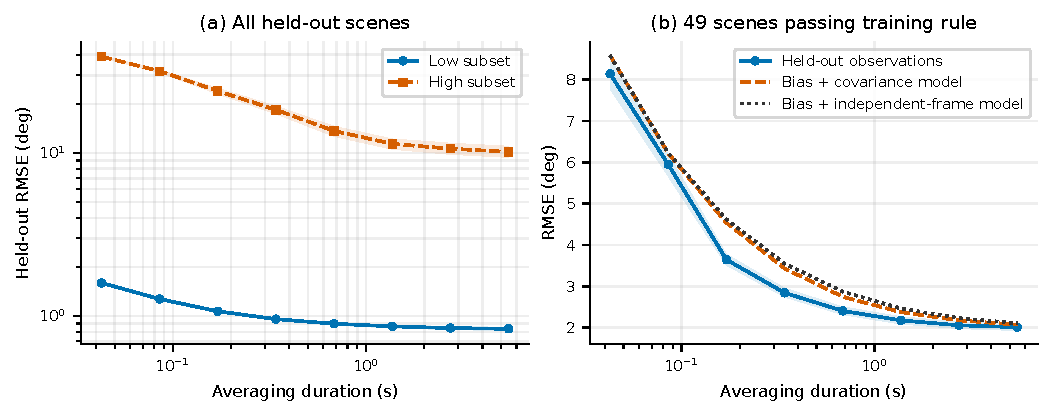
\includegraphics[width=\textwidth]{fig5_heldout_averaging.pdf}
	\caption{Temporal averaging evaluated on new recordings. (a) All non-overlapping circular block averages from the 72 held-out scenes, separated into the low-reverberation/centred and high-reverberation/offset subsets. Each subset contains 180 recordings and contributes $180\times128/N$ estimates at block length $N$. (b) Results for the 49 scenes that met the criteria applied to the estimation recordings. Model curves are predictions; shaded bands are 95\% bootstrap intervals from complete test recordings. Estimation and test recordings are independent.}
	\label{fig:averaging}
\end{figure*}

\subsection{Timing-precision bound for the array}

I use an additional calculation to relate microphone arrival-time error to error in the fitted direction. Let $B$ form the pairwise differences between the three arrivals and let $M$ contain the microphone coordinates, with $A=BM$. If $\boldsymbol\epsilon$ contains the microphone arrival errors, the fitted direction changes by
\begin{equation}
	\delta\widetilde{\mathbf u}
	=
	J\boldsymbol\epsilon,
	\qquad
	J=-cA^+B,
\end{equation}
where $A^+$ is the Moore--Penrose pseudoinverse. This form retains the dependence created when one microphone appears in multiple pairs.

Suppose every arrival error satisfies $|\epsilon_i|\leq h$. The norm of this linear mapping is convex over the error box, meaning its maximum can be found from the eight corner combinations $\epsilon_i=\pm h$:
\begin{equation}
	\rho
	=
	\max_{\epsilon_i\in\{-h,h\}}
	\left\|J\boldsymbol\epsilon\right\|.
\end{equation}
If $\rho<\|\widetilde{\mathbf u}\|$, every admissible perturbation satisfies the conservative angular bound
\begin{equation}
	|\delta\theta|
	\leq
	\arcsin\!\left(
	\frac{\rho}{\|\widetilde{\mathbf u}\|}
	\right).
	\label{eq:bound}
\end{equation}
Under the same condition, evaluating angular change at all eight corners gives an exact box bound. Their linear image is a convex polygon that does not contain the origin, so the angular extremes occur at its vertices. Figure~\ref{fig:precision}(a) compares this exact box bound with the conservative disk bound in equation~\ref{eq:bound}.

For the centred equilateral array and a plane wave, $\rho=4ch/(3R)$ and $\|\widetilde{\mathbf u}\|=1$. For $0<\eta<90^\circ$, a sufficient condition for keeping the angular change at most $\eta$ is therefore
\begin{equation}
	h
	\leq
	\frac{3R}{4c}\sin\eta.
\end{equation}
At $R=0.05$ m and $\eta=0.5^\circ$, this sufficient condition allows no more than $0.954\,\mu$s absolute error in each arrival time. The result applies to ideal arrivals passed through the direction solver. It is not a necessary sampling-rate requirement and does not guarantee the accuracy of noisy GCC-PHAT estimates.

I compared every observed angular change with its calculated bound. None of the 34,560 rounded-arrival cases exceeded it. A further 12,000 random perturbations, including unequal triangles and an independent scalar solution, also produced no violations. Figure~\ref{fig:precision}(a) measures each change relative to the estimate from exact spherical arrivals. Any difference between that reference and the true source direction is a separate finite-distance effect.

\subsection{Additional geometries and comparison with SRP-PHAT}

On the fixed 24-scene subset, GCC-PHAT produced an RMSE of $22.413^\circ$ in the base condition. The independent sensitivity recordings gave $23.729^\circ$ for the rotated array, $19.644^\circ$ for the unequal triangle, $23.643^\circ$ for unequal walls and $42.054^\circ$ for the narrower-band source (Figure~\ref{fig:precision}(b)). Since these conditions use new random recordings, their differences from the base value are neither paired causal effects nor evidence of an optimised geometry. In the narrower-band condition, part of the fixed estimator passband contains noise without source energy. Its result combines the effect of a narrower source spectrum with this estimator-band mismatch.

The SRP-PHAT comparison reuses the same base recordings as GCC-PHAT. Its RMSE was higher, $30.262^\circ$ against $22.413^\circ$, but fewer estimates exceeded $5^\circ$: 28.62\% against 30.57\%. The matched SRP-minus-GCC difference in mean squared error was $413.473\,\mathrm{deg}^2$ $[268.788,561.435]\,\mathrm{deg}^2$. These summaries describe different parts of the distribution. A method can cross the selected threshold less often while still producing more extreme errors. This restricted comparison does not establish a general ranking between the methods.

\begin{figure*}[t]
	\centering
	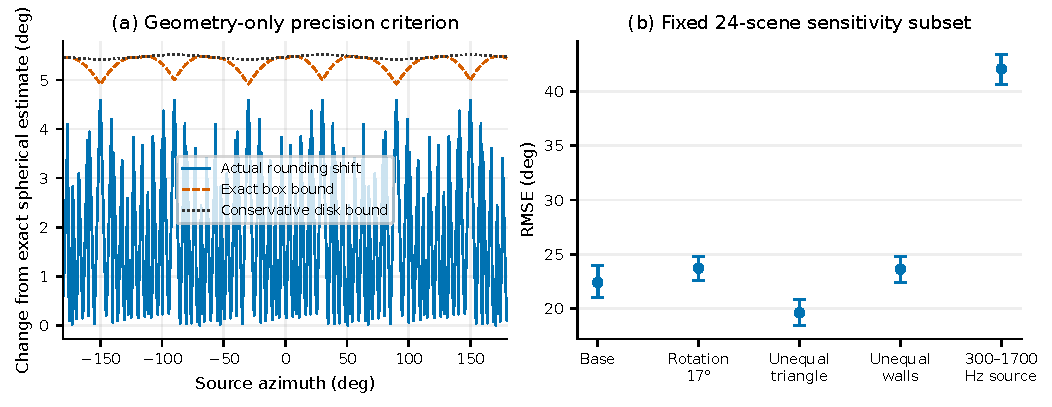
\includegraphics[width=\textwidth]{fig6_precision_sensitivity.pdf}
	\caption{Timing precision and sensitivity conditions. (a) Analytical changes caused by arrival-time rounding and their bounds at 48 kHz, with an array radius of 0.05 m and a source distance of 1.5 m. Changes are measured relative to the estimates obtained from exact spherical arrivals. (b) RMSE and record-bootstrap intervals for five conditions on the fixed 24-scene subset. In the narrower-source-band condition, the acquisition and estimator bands remain 300--3400 Hz.}
	\label{fig:precision}
\end{figure*}

\section{Discussion and practical implications}

The first practical result is that subsample arrival construction changes the direction estimate. Fractional-delay methods represent arrivals that lie between discrete sample times \citep{laakso}. Replacing them with nearest-sample values increased error even after waveform generation and GCC-PHAT processing \citep{knapp}. Rounding was not the largest error source in reflective rooms, but its effect was large enough to distort an evaluation of a compact array.

Source history had a much larger effect on the first frame containing reflections. In an image-source simulation \citep{allen}, zeroing the signal before acquisition removes contributions that would have arrived from earlier emissions. The onset frame is therefore a different acoustic condition, not simply an earlier sample of steady operation. A continuous-operation simulation needs enough prehistory to cover both the retained room response and the acquisition-filter transient. If source onset is the actual application of interest, then the onset condition should remain, but it must be identified as such.

The numerical correction also exposed a less obvious dependency between response duration and image extent. A long response window cannot recover paths that were never generated because the image extent was too small. Spectral agreement alone is not enough either, since a peak-based estimator may still select a different correlation maximum. Checking the response and direction together revealed the limitation in the original room calculation and led to the corrected campaign used here.

Temporal averaging reduced error without changing the per-frame localizer. Its extra cost is the accumulation of circular components and a longer observation interval, reaching 5.461 s for the largest block. The benefit was strongly scene-dependent. Averaging can suppress fluctuations between frames, but it cannot be expected to remove persistent bias from a mismatched wavefront model or repeated selection of the wrong correlation peak. I assessed the covariance model only where the small-error criteria were met, while keeping every scene in the empirical curves. Its weaker agreement at shorter durations makes it unsuitable as a precise general prediction. These stationary-source results also say nothing about moving-source tracking, and I did not measure processing time, memory or energy use.

The matched SRP-PHAT comparison \citep{dibiase} shows why RMSE should not be reported alone. SRP-PHAT crossed the selected error threshold less often but had a larger RMSE because its largest errors contributed more heavily. The comparison covers one restricted subset and fixed implementations of both estimators, so it does not support a universal claim that either method is better.

The physical interpretation remains limited by the simulation itself. The microphones are ideal and matched, excluding gain mismatch, clock drift, calibration error and device-specific frequency response. The source is stationary band-limited Gaussian noise rather than speech or machinery. Reflections are specular and frequency-independent, with no measured scattering or microphone directivity. The main study uses one array size and one source distance, although the analytical timing checks cover a wider range. Only horizontal direction is estimated, and neither the source nor the array moves during a recording.

The bootstrap intervals use five independent recordings per scene: 32-frame recordings for the main and matched-condition studies, plus separate 128-frame test recordings for averaging. They describe resampling variation within the fixed simulated scenes, not calibrated population intervals for arbitrary rooms. I did not assess their coverage independently, and the scene-level intervals have limited resampling support. Three rectangular geometries cannot represent the range of real rooms either. Transfer to physical microphones and real acoustic environments must be tested in a measured-room experiment.

\section{Conclusion}

This work separates three effects that are easily mixed together in a sound-localization simulation: arrival-time rounding, source startup and reflected propagation. Nearest-sample rounding increased direct-path error even after full waveform processing. Beginning acquisition at source onset created a temporarily easier reflected-sound condition than continuous operation. Temporal averaging reduced error on independent recordings, although the error left behind still depended on the scene.

Independent calculations and refinement tests establish the numerical resolution of these comparisons for the cases tested. The geometry-based timing bound provides another check on ideal arrival perturbations while retaining the dependence between microphone pairs. More practically, the results show why a compact-array evaluation must report how arrivals are discretised and whether the simulated source is at onset or in steady operation. The study does not establish hardware accuracy, universal estimator superiority or a general relation between reverberation and localization error.


\bibliographystyle{unsrtnat}
\begingroup\interlinepenalty=10000
\bibliography{references}
\endgroup
\end{document}
